\documentclass[12pt]{scrartcl}
\usepackage{ucs}
\usepackage[utf8x]{inputenc}
\usepackage[T1]{fontenc}
\usepackage[ngerman]{babel}
\usepackage{graphicx}
\usepackage{float}
\usepackage{listings}
\usepackage[table,xcdraw]{xcolor}
\usepackage[automark]{scrpage2}
\usepackage[normalem]{ulem}
\useunder{\uline}{\ul}{}
\pagestyle{scrheadings}
\clearscrheadfoot
\ifoot[]{\author}
\ofoot[]{\pagemark}

%\title{Modul zum Import verschiedener Dateiformate}
%\author{Mark Unger und Siegfried Kienzle}
%\date{Konstanz, den \today{}}



\begin{document}

\begin{titlepage}
	\centering
	
\includegraphics[width=0.5\textwidth]{HTWG}\par\vspace{2.5cm}
	\vspace{1cm}
	{\scshape\Large Handbuch für\par}
	\vspace{1.5cm} 
	{\scshape\bfseries Modul zum Import verschiedener Dateiformate\par}
	\vspace{2cm}
	{\Large\itshape Mark Unger und Siegfried Kienzle\par}
	\vfill

% Bottom of the page
	{\large \today\par}
\end{titlepage}


\newpage

\begin{center}
\section*{Erklärung}
Die in diesem Projekt verwendete Software unterliegt den 
rechtlich jeweiligen Bestimmungen der einzelnen Organisationen und Firmen. 
\vfill
\end{center}

\newpage
\tableofcontents
\newpage

\section{Modul}
\label{sec:modul-einleitung}

\subsection{Über die Software}
\label{sec:software-einleitung}
Dieses Modul dient zur Extrahierung von Text aus Dateien. 
Sie können dieses Modul für folgende Endungen verwenden:
\begin{itemize}
	\item .doc
	\item .docx
	\item .odt
	\item .pdf
	\item rtf
\end{itemize}
Es wurde für Python 3.4.3 entwickelt und unter 
Ubuntu 14.04.05 LTS getestet. Zur Installation liegt 
ein Bash-Script vor. 

\subsection{Über das Handbuch}
\label{sec:handbuch-einleitung}
Dieses Handbuch beschreibt die Installation und die Handhabung
mit dem Modul. 


\newpage
\section{Grundlagen}
\label{sec:grundlagen}
\subsection{Installation}
\label{sec:grundlagen-installation}
\begin{enumerate}

\item Installationsscript mittels ./inst.sh aufrufen:
\newline
\begin{figure}[htbp]
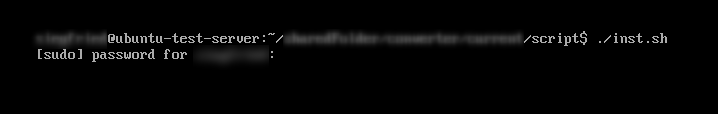
\includegraphics[width=1.0\textwidth]{schritt1}\par\vspace{0.5cm}
\caption{Nach Aufruf des Installationscriptes ./inst.sh}
\label{fig:script1}
\end{figure}
\item sudo-Passwort eintippen und die Enter-Taste drücken.
\item Es werden nun einige Abhängigkeiten installiert, die 
zur Ausführung dieses Moduls benötigt werden.
\newpage
\item Geben Sie nun den Pfad an, in den das Modul installiert werden soll.
Sollte der Pfad nicht existieren, werden Sie wie in Abbildung 4 gefragt
ob der Pfad erstellt werden soll. 
Existiert der Pfad, entfallen die Schritte 6 bis 8. 
\begin{figure}[htbp]
\centering
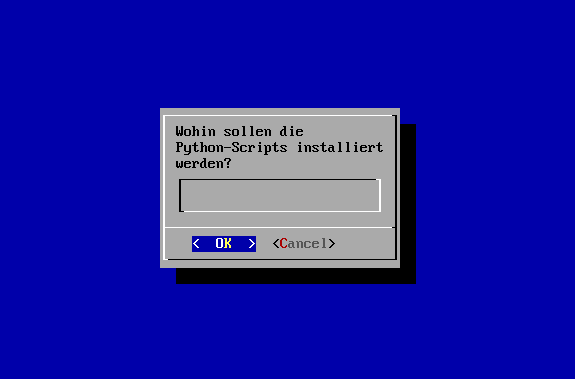
\includegraphics[width=0.6\textwidth]{schritt2}\par\vspace{0.5cm}
\caption{Nach Aufruf des Installationscriptes ./inst.sh}
\label{fig:script2}
\end{figure}
\begin{figure}[htbp]
\centering
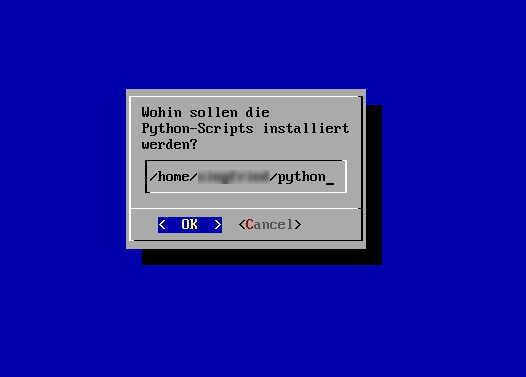
\includegraphics[width=0.6\textwidth]{schritt3}\par\vspace{0.5cm}
\caption{Nach Eingabe des Installationspfads}
\label{fig:script3}
\end{figure}
\item Wenn der OK-Button blau hinterlegt ist, können Sie mit
der Enter-Taste den Pfad bestätigen. 
\newpage
\item Sollte kein Pfad existieren, erscheint folgendes Fenster:
\begin{figure}[htbp]
\centering
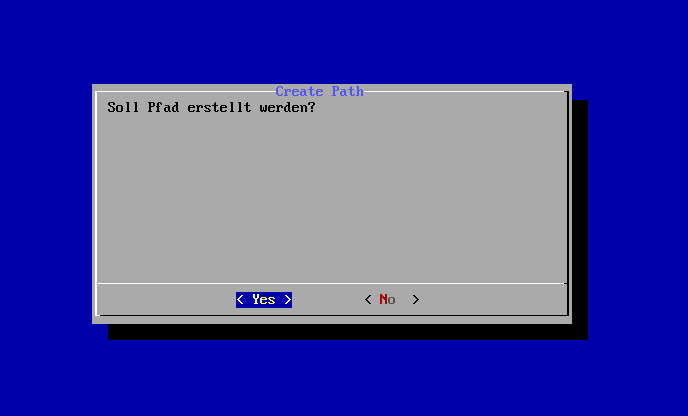
\includegraphics[width=1.0\textwidth]{schritt4}\par\vspace{0.5cm}
\caption{Pfad erstellen?}
\label{fig:script4}
\end{figure}
\item Wählen Sie nun mit den Pfeiltasten aus, ob Sie den Pfad erstellen möchten
oder nicht und drücken Sie dann die Enter-Taste.
\begin{figure}[htbp]
\centering
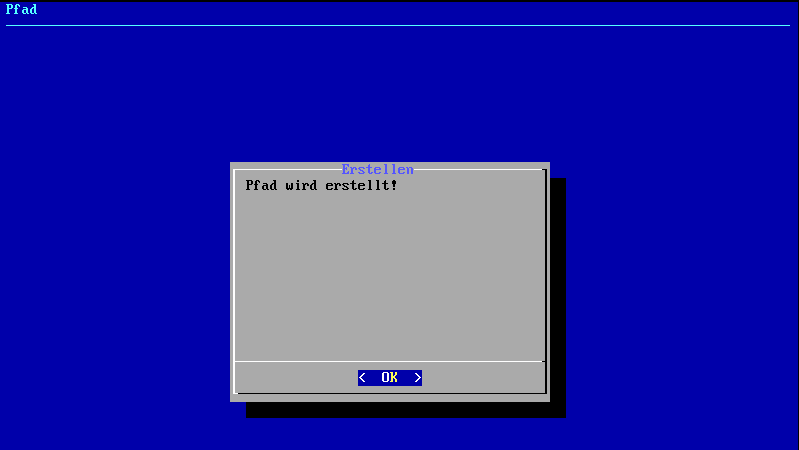
\includegraphics[width=0.8\textwidth]{schritt5}\par\vspace{0.5cm}
\caption{Pfad wurde erstellt}
\label{fig:script5}
\end{figure}
\newpage
\item Es wurde nun der Pfad erstellt. Drücken Sie nun die Enter-Taste, um die Dateien
in das entsprechend vorher erstellte Verzeichnis, zu entpacken.
\begin{figure}[htbp]
\centering
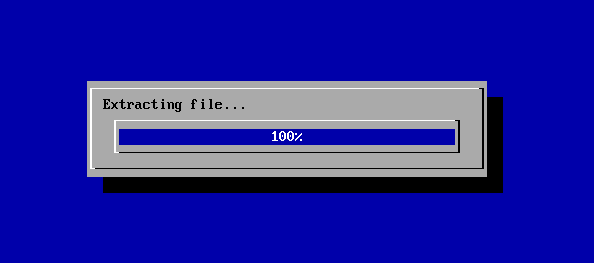
\includegraphics[width=0.8\textwidth]{schritt6}\par\vspace{0.5cm}
\caption{Pfad wurde erstellt}
\label{fig:script6}
\end{figure}
\item Die Installation ist nun abgeschlossen. Prüfen Sie nun 
bitte ob alle Dateien installiert wurden. Eine genaue Auflistung finden
Sie unter dem Punkt 2.3.
\end{enumerate} 
\subsection{Bestandteile Installationspaket}
\label{sec:installationsbestandteile}
\begin{table}[H]
\centering
\label{installationsbestandteile}
\begin{tabular}{|l|l|}
\hline
\rowcolor[HTML]{9B9B9B} 
Datei      & Beschreibung                                                      \\ \hline
inst.sh    & Bash-Script für die Ausführung als Super-User (sudo) unter Ubuntu \\ \hline
ubuntu.sh  & Bash-Script für die Installation unter Ubuntu                     \\ \hline
moduls.tar & Tar-Datei, die die Python-Module enthält                          \\ \hline
\end{tabular}
\caption{Bestandteile Installationspaket}
\end{table}
\subsection{Modulbestandteile}
\label{sec:modulbestandteile}
\begin{table}[H]
\centering
\label{modulbestandteil}
\begin{tabular}{|l|l|}
\hline
\rowcolor[HTML]{9B9B9B} 
Datei           & Verwendung                           \\ \hline
convertToTxt.py & Datei die für das Extrahieren aufgerufen wird \\ \hline
extractTxt.py   & Hauptdatei für die Extrahierung      \\ \hline
docTxt.py       & Modul für die Dateiendung doc        \\ \hline
docxTxt.py      & Modul für die Dateiendung docx       \\ \hline
odtTxt.py       & Modul für die Dateiendung odt        \\ \hline
pdfTxt.py       & Modul für die Dateiendung pdf        \\ \hline
rtfTxt.py       & Modul für die Dateiendung rtf        \\ \hline
\end{tabular}
\caption{Modulbestandteile}
\end{table}
\newpage
\subsection{Erste Schritte}
\label{sec:first-steps}
\subsubsection{Genereller Aufruf}
\label{sec:first-steps-general}
Im Allgemeinen wird das Modul wie folgt aufgerufen:
%ersteSchritte001
\begin{figure}[htbp]
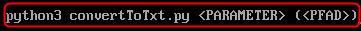
\includegraphics[width=1.0\textwidth]{ersteSchritte001}\par\vspace{0.25cm}
%\caption{Aufruf der Hilfe mittels -h}
\label{fig:ersteSchritteGeneral001}
\end{figure}
\newline
Dabei sollte <PARAMETER> durch einen Parameter aus Tabelle 3 ersetzt werden. Beim Parameter -p bzw. -{}-process sollte dann zusätzlich <PFAD> (das hier in runden Klammern steht) durch den Pfad der Datei, aus der der Text extrahiert werden soll, ersetzt werden. 
Außerdem ist zwingend darauf zu achten, dass das Modul mit python3 aufgerufen wird.
\begin{table}[H]
\begin{center}
\label{params}
\begin{tabular}{|l|l|l|}
\hline
\rowcolor[HTML]{C0C0C0} 
Parameter (kurz) & Parameter (lang) & Erklärung                                                                                                                              \\ \hline
-h               & -{}-help           & Zeigt die Hilfe an                                                                                                                     \\ \hline
-p               & -{}-process        & Führt die Textextrahierung durch.  \\ \hline
-v				 & ------------------ & Verbose-Mode: Gibt den Text auf Konsole aus. \\ \hline
-o               & -{}-output         & Parameter für die Ausgabedatei.\\
				 &					  &	Nur anwendbar mit Argument -p bzw. -{}-process \\ \hline
\end{tabular}
\caption{Parameterübersicht}
\end{center}
\end{table}

Beispielaufrufe finden Sie weiter unten in diesem Kapitel. 
\newpage
\subsubsection{Extrahieren von Text auf Konsole}
\label{sec:first-steps-extraction-console}
Zum Extrahieren von Text tippen Sie einfach	
python3 convertToTxt.py -p <PFAD ZUR GEWÜNSCHTEN DATEI> -v oder python3 convertToTxt.py -{}-process <PFAD ZUR GEWÜNSCHTEN DATEI> -v.
Als Beispiel sehen Sie im folgenden wie Text aus einer DOCX-Datei extrahiert wird:
\begin{figure}[htbp]
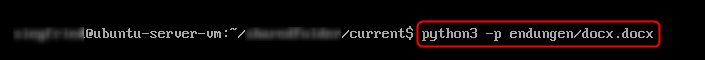
\includegraphics[width=1.0\textwidth]{ersteSchritteExtract001}\par\vspace{0.25cm}
%\caption{Aufruf der Hilfe mittels -h}
\label{fig:ersteSchritteExtract001}
\end{figure}
\begin{center}
oder
\end{center}
\begin{figure}[htbp]

\includegraphics[width=1.0\textwidth]{ersteSchritteExtract002}\par\vspace{0.25cm}
%\caption{Aufruf der Hilfe mittels -h}
\label{fig:ersteSchritteExtract002}
\end{figure}
\begin{figure}[htbp]
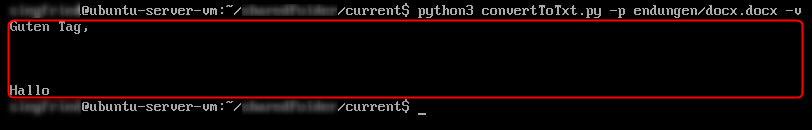
\includegraphics[width=1.0\textwidth]{ersteSchritteExtract003}\par\vspace{0.25cm}
\caption{Beispielausgabe von docx}
\label{fig:ersteSchritteExtract003}
\end{figure}
\newpage
\subsubsection{Extrahieren von Text in eine Datei}
\label{sec:first-steps-extraction-file}
\newpage
\subsubsection{Hilfe aufrufen}
\label{sec:first-steps-help}
Zum Aufrufen der Hilfe einfach wie im folgenden Bild den Parameter -h bzw. -{}-help eingeben.
\newline
\begin{figure}[htbp]
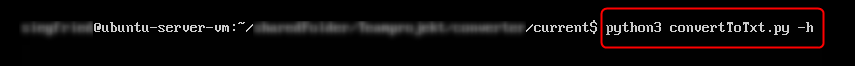
\includegraphics[width=1.0\textwidth]{ersteSchritte1}\par\vspace{0.25cm}
%\caption{Aufruf der Hilfe mittels -h}
\label{fig:ersteSchritte1}
\end{figure}
\begin{center}
oder
\end{center}
\begin{figure}[htbp]
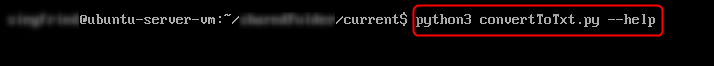
\includegraphics[width=1.0\textwidth]{ersteSchritte2}\par\vspace{0.5cm}
%\caption{Aufruf der Hilfe mittels - -help}
\label{fig:ersteSchritte2}
\end{figure}
Die Ausgabe sollte wie folgt aussehen:
\begin{figure}[htbp]
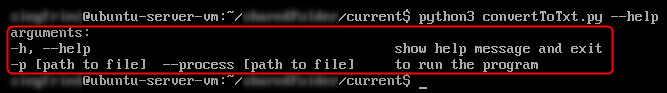
\includegraphics[width=1.0\textwidth]{ersteSchritte3}\par\vspace{0.5cm}
%\caption{Aufruf der Hilfe mittels - -help}
\label{fig:ersteSchritte3}
\end{figure}
\newpage
\section{Technischer Hintergrund}
\label{sec:technical-background}
\subsection{Aufbau}
\label{sec:technical-background-aufbau}
\subsection{Verwendete Fremdsoftware}
\label{sec:technical-background-fremdsoftware}
\newpage
\section{Kontaktdaten}
\label{sec:kontaktdaten}
\begin{table}[H]
%\centering
\label{kontaktdaten}
\begin{tabular}{|l|l|}
\hline
\rowcolor[HTML]{9B9B9B} 
Name              & E-Mail                   \\ \hline
Mark Unger        & mrk.unger@gmail.com      \\ \hline
Siegfried Kienzle & siegfried.kienzle@gmx.de \\ \hline
\end{tabular}
%\caption{Kontaktdaten}
\end{table}
\end{document}